\documentclass{article}

\usepackage{listings} % for including MATLAB code
\usepackage{graphicx} % for including images

\title{80846 - Report - 2nd}
\author{GU JUN, 6132230056-4}
\date{\today}

\begin{document}

\maketitle

\section*{Introduction}

The following content will be organized in the following way: Problem Statement, Simulink model, Source codes for RobotDynamics and controller blocks, Simulation results, and Explanation.

\section*{Problem Statement}

According to the class, we are required to complete two things: \\
\textbf{1. Robot dynamics for 2-DOF robot arm.} \\
\textbf{2. passivity-based Controller.}

% model of the system
\section{Simulink Model}
See the Figure \ref{fig:model} below. The whole system inclues two blocks: RobotDynamics and Controller.
Compared with the model before, I change the RobotDynamics part to a subsystem to make the whole model looks more clear.\\
\begin{figure}[ht]
    \centering
    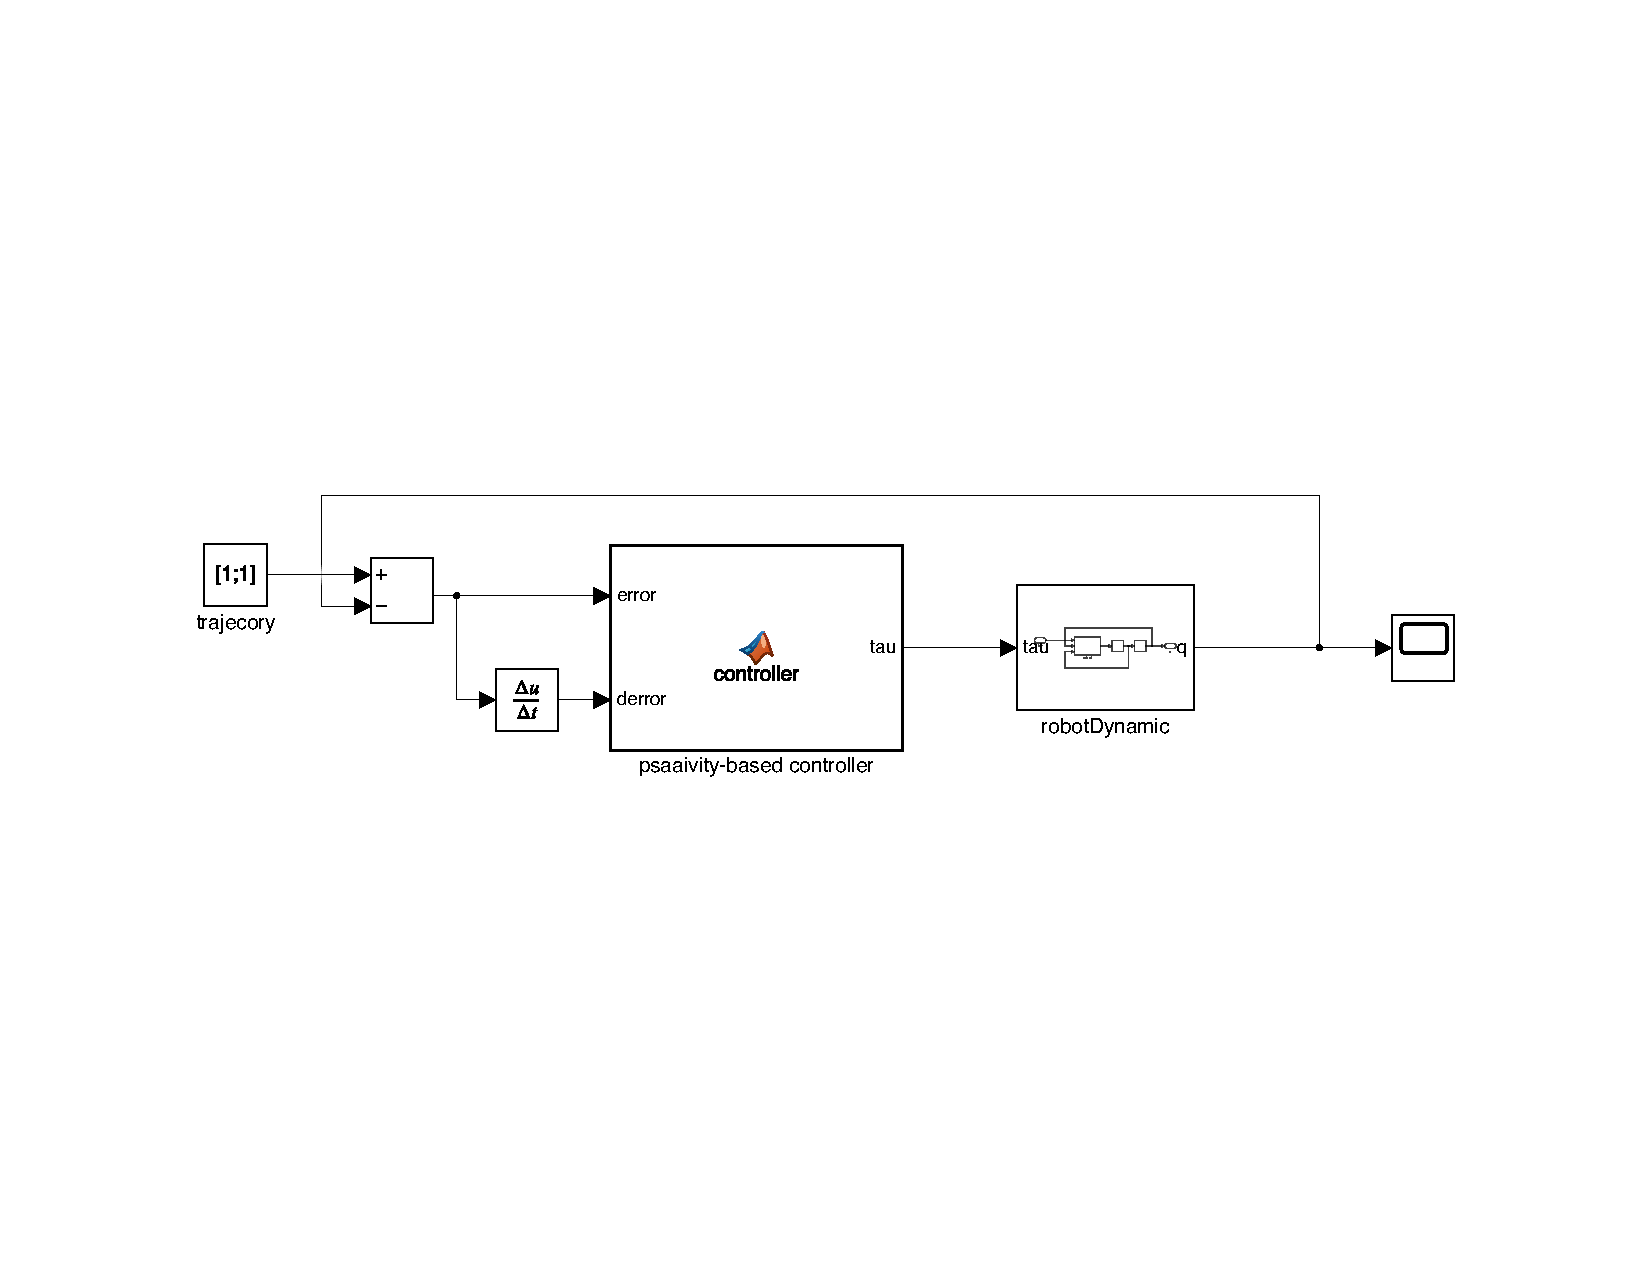
\includegraphics[width=0.9\textwidth]{figures/model.pdf}
    \caption{Simulink Model of whole system}
    \label{fig:model}
\end{figure}

% formulas and source codes
\section{Formulas and Source Codes}
This part inclues the formulas and source codes for RobotDynamics and Controller blocks.
\subsection*{RobotDynamics}
The robot dynamics is calculated by the following formula:
    \begin{equation}
        M \ddot{q} + h = \tau
    \end{equation}

    \begin{equation}
        F = L \tau
    \end{equation}

    \begin{equation}
        F = \frac{d}{dt} \left[ \frac{\partial\mathcal{L}}{\partial \dot{q}}\right] - \frac{\partial\mathcal{L}}{\partial q}
    \end{equation}
    \begin{equation}
        \mathcal{L} = \mathcal{K} - \mathcal{P}
    \end{equation}
where $F$ is force vector, $\mathcal{L}$ is the Lagrangian, $\mathcal{K}$ is the kinetic energy, $\mathcal{P}$ is the potential energy.\\

The source code is shown below:
\begin{lstlisting}[language=Matlab, basicstyle=\small\ttfamily]
function ddq = robot(tau, q, dq)

    I1 = 0.05;
    m1 = 1.5;
    lg1 = 0.2;
    
    I2 = 0.01;
    m2 = 0.5;
    lg2 = 0.2;
    
    g = 9.8;
    % g = 0;
    
    a1 = I1 + I2 + m2 * lg1 * lg1;
    a2 = m2 * lg1 * lg2;
    a3 = I2 ;
    
    L = [lg1, 0;
            0, lg2];
    
    M = L * [a1 + 2 * a2 * cos(q(2)), a3 - a2 * cos(q(2));
             a3 + a2 * cos(q(2)), a3 / lg2];
    
    h = L * [-a2 * sin(q(2)) * (2*dq(1)*dq(2) + dq(2)*dq(2)) 
             - (m1 + m2) * lg1 * g * sin(q(1));
             -a2 * sin(q(2)) * dq(1) * dq(2) 
             - m2 * lg2 * g * sin(q(1) + q(2))];
    
    ddq = M \ (tau - h);
    
\end{lstlisting}

\subsection*{Controller}

The controller is calculated by the following formula:
\begin{equation}
    \tau = k_p \cdot error + k_d \cdot \frac{d}{dt}error
\end{equation}


The source code is shown below:
\begin{lstlisting}[language=Matlab,  basicstyle=\small\ttfamily]
    function tau = controller(error, derror)

    kp = [10, 0;
           0, 4];
    
    
    kd = [1, 0;
            0, 0.3];
    
    tau = kp * error + kd * derror;
\end{lstlisting}

\section{Simulation Results}

After some tuning of the gains, I got the following Figure \ref{fig:result_plot}. \\
As you can see, the angles didn't follow the trajecty well, the error is existing after the results converged.\\
I try to tune the gains, but the error is still existing.\\ 
\begin{figure}[ht]
    \centering
    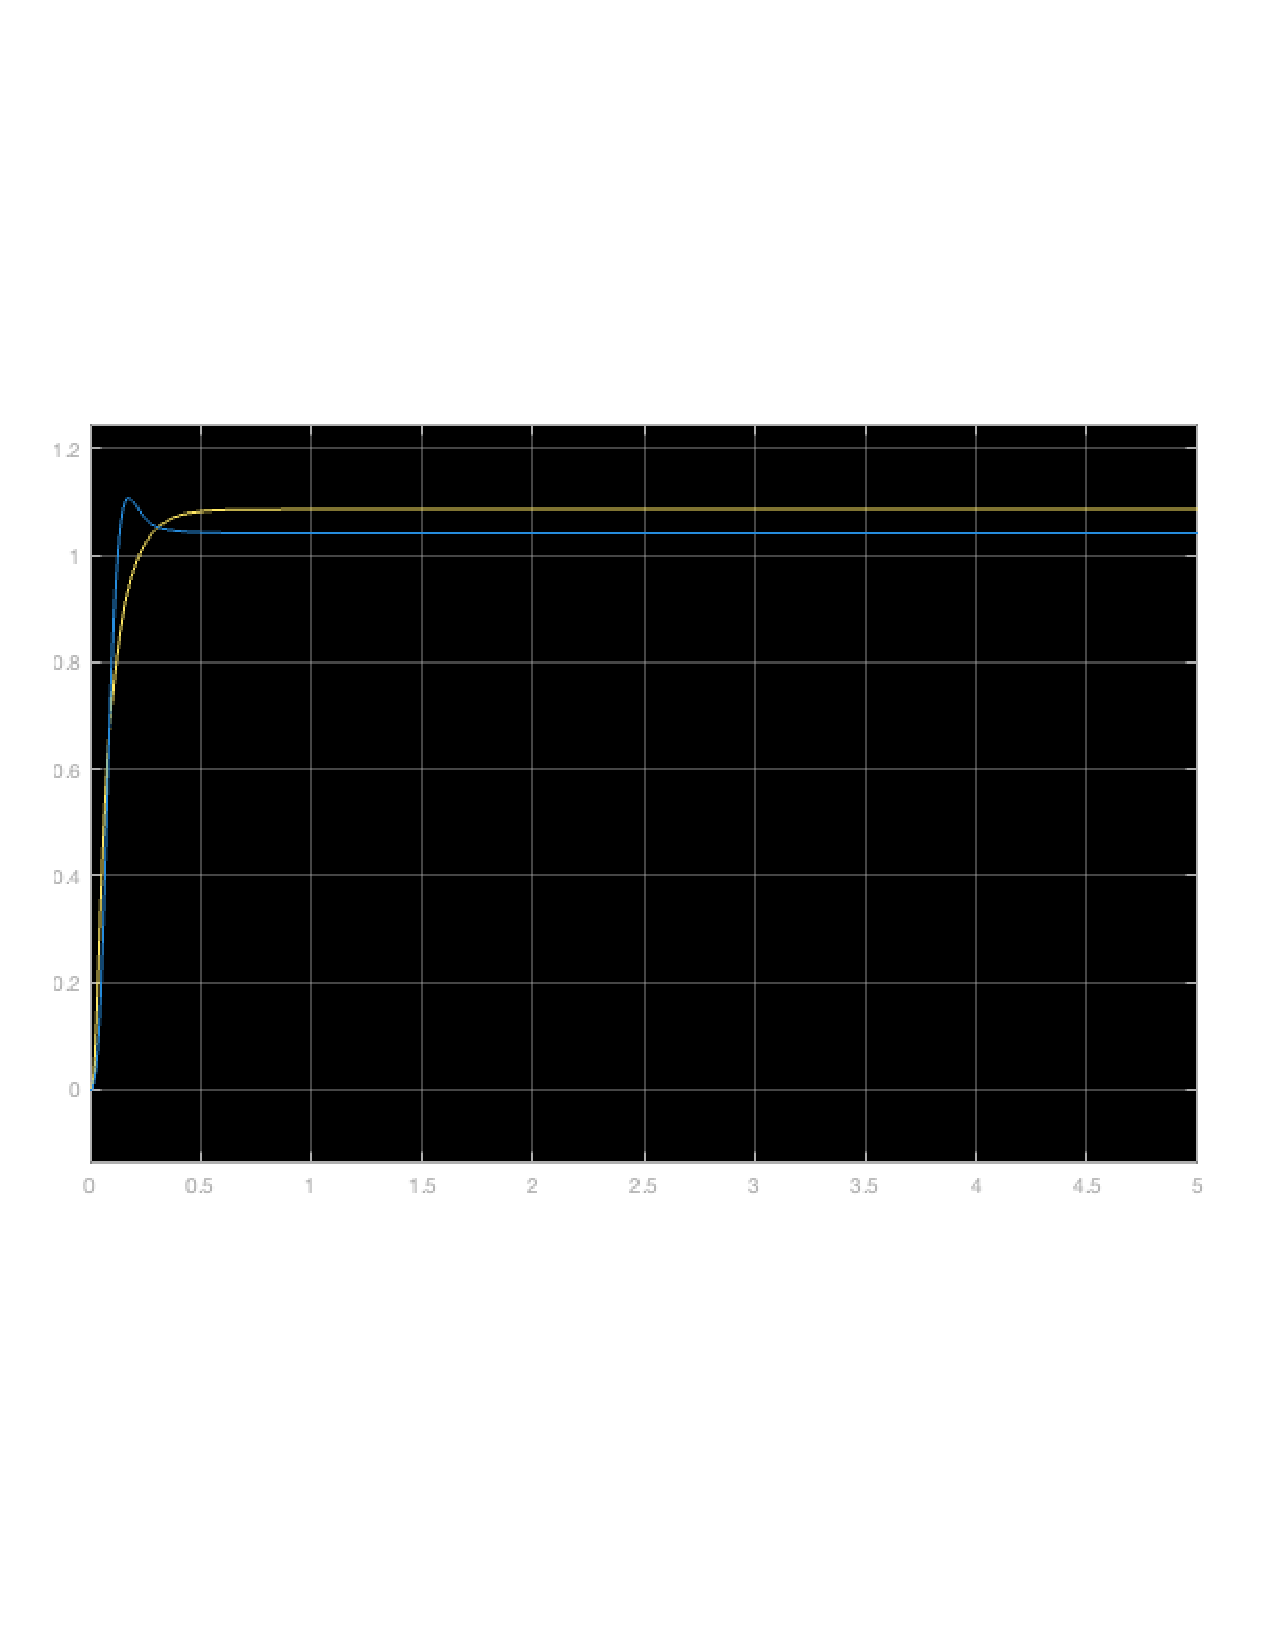
\includegraphics[width=0.8\textwidth]{figures/result.pdf}
    \caption{Result Plot, error still existing after simulation time.}
    \label{fig:result_plot}
\end{figure}

\newpage
\section{Explanation}
According to the formulas and source codes, most parts are very clear.
I calculated the robot dynamics accoring to its dynamics, and the controller part is very simple.
However, the error is still existing after the simulation time. I think there are two reasons: \\
\textbf{1. The gains are not suitable.} \\
\textbf{2. The system is not linear}



\end{document}